\chapter{Turingmaschinen}
\index{Turingmaschine}
\index{Church-Turing-These}
\newcommand{\blank}{b}
%
% Turingmaschinbeispiele:
%   {Zahl1, Zahl2, Zahl3} mit Zahl* in [-8 bis 7]... ermittle Minimum
Alan Turing (\life{1912}{1954}) machte sich viele Gedanken rund um mathematische Beweise und mechanische Prozesse. Er fragte sich, ob eine automatisierte Beweisführung von mathematischen Formeln möglich ist und konzipierte hierfür ein Maschinenkonzept. Die ,,a-machine`` (oder heutzutage als ,,Turingmaschine`` bezeichnet) wurde zum Referenzmodell der Theoretischen Informatik, welche auf einem praktikablen Weg zeigt, wo die Grenzen von Berechenbarkeit liegen und was automatisiert werden kann. Die Church-Turing-These behauptet, dass auch andere Konzepte wie das $\lambda$-Kalkül (welches zur selben Zeit entstanden ist) bezüglich Berechenbarkeit äquivalent sind.

\begin{quotation}
 Die Klasse der intuitiv berechenbaren Funktionen ist genau die Klasse der turing-berechenbaren (dh. durch eine Turingmaschine berechenbare) Funktionen. \\
 ---Die Church-Turing-These
\end{quotation}
%
\section{Definition}
%
Eine Turingmaschine ist formal betrachtet ein 7-Tupel.
\begin{equation}
  TM = (Q, \Sigma, \Gamma, \delta, q_0, \blank, F)
\end{equation}
%
\begin{description}
 \item[$Q$] Eine Menge an Zuständen, die die Turingmaschine annehmen kann.
 \item[$\Sigma$] Eine Menge an Zeichen, welche auf dem Band initial verwendet werden (Blankzeichen exklusive).
 \item[$\Gamma$] Eine Menge an Zeichen, die auf dem Band verwendet werden können (Blankzeichen inklusive).
 \item[$\delta$] Die Übergangsfunktion.
 \item[$q_0$] Ein Anfangszustand der TM.
 \item[$\blank$] Das Blanksymbol, welches den Initialzustand unbeschriebener Stellen beschreibt.
 \item[$F$] Eine Menge von Zuständen. Wird einer dieser Zustände erreicht, hält die Turingmaschine an (,,Endzustände``).
\end{description}
%
Dabei gelten folgende Relationen zwischen den Elementen:
\begin{equation}
  \blank \notin \Sigma,  \mathspace  \blank \in \Gamma
\end{equation}
\begin{equation}
  \Sigma \subseteq \Gamma,  \mathspace  \blank \in \Gamma
\end{equation}
\begin{equation}
  q_0 \in Q
\end{equation}
\begin{equation}
  F \subset Q
\end{equation}

\section{Funktionsweise}
%
\begin{figure}[ht]
 \begin{center}
  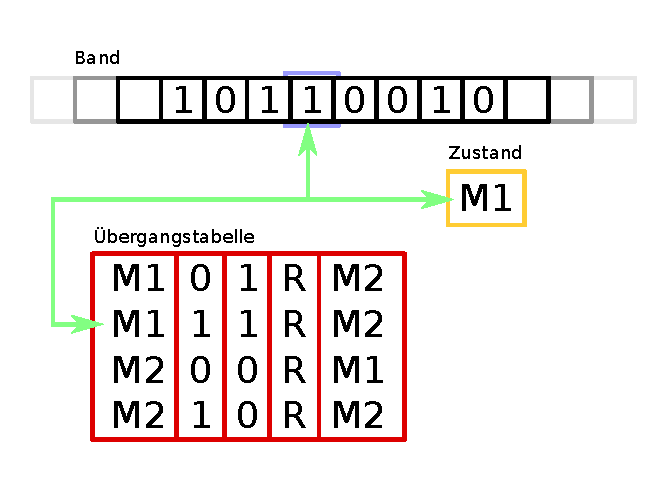
\includegraphics{img/turingmachine_visualization.pdf}
  \caption{Die Funktionsweise einer Turingmaschine visualisiert}
  \label{fig:tm_vis}
 \end{center}
\end{figure}
%
In Abbildung~\ref{fig:tm_vis} ist der Aufbau einer Turingmaschine visualisiert. Die Turingmaschine besitzt ein unendlich langes Band (schwarz) auf welchem Zeichen aus dem Alphabet $\Gamma$ stehen. Der Cursor (blau) befindet sich an einer bestimmten Stelle auf diesem Band und liest und schreibt Zeichen. Basierend auf der Information in welchem Zustand (orange) sich die Turingmaschine befindet und welches Zeichen gelesen wurde, wird eine Zeile in der Übergangstabelle (rot) ausgewählt.

Die Turingmaschine besitzt eine initiale Konfiguration. Als Konfiguration bezeichnet man das Tupel (Zustand, Band, Cursor). Die abgebildeten Turingmaschine befindet sich in einem Zustand M1, auf dem Band befinden sich die Zeichen 10110010 (aus dem Alphabet $\Sigma$) und der Cursor ist links der Mitte positioniert. Dies sei unsere initiale Konfiguration und weitere Konfigurationen lassen sich jetzt durch schrittweise Ausführung der Instruktionen ableiten. \\
Aufgrund der Konfiguration können wir jetzt in der Übergangstabelle nachschlagen, welche Instruktion ausgeführt werden soll. Eine Zeile der Spalte besteht dabei aus 5 Werten: Ausgangszustand, gelesenes Zeichen, geschriebenes Zeichen, Bewegung und Endzustand. Dies bedeutet in Zeile~2 stimmt die Konfiguration mit den Werten überein: Wir befinden uns im Zustand M1 (ja, in diesem befinden wir uns gerade) und lesen das Zeichen ,,1`` (ja, wurde vom Cursor gelesen). Dementsprechend ist eine ,,1`` an diese Position am Band zu schreiben, nach rechts (,,R``) zu fahren und in den Zustand ,,M2`` zu wechseln. Wenn wir den nachfolgenden Schritt beobachten, wird die Zeile 3 ausgeführt: Im Zustand ,,M2`` wurde das Zeichen ,,0`` gelesen, wird das Zeichen ,,0`` geschrieben, der Cursor nach rechts (,,R``) bewegt und in den Zustand ,,M1`` gewechselt.

Erreicht die Turingmaschine einen der definierten Endzustände, wird die Eingabe als ,,akzeptiert`` (Ja) interpretiert. Kommt die Turingmaschine in einen undefinierten Zustand, wird die Eingabe ,,abgelehnt`` (Nein).

Durch das Wechseln von Zuständen und das Speichern von Zeichen auf dem Band können Daten verarbeitet werden. Den Input und Output eines ablaufenden Algorithmus' bildet die Initial- und Endkonfiguration der Turingmaschine. Die Logik bzw. das Programm ist in der Übergangstabelle kodiert.

\section{Ein einfacher Algorithmus}
%
Gegeben sei eine Turingmaschine. Auf dem Band befindet sich eine beliebige Sequenz von 0en und 1en, die nicht durch ein Blanksymbol unterbrochen wird. Gesucht ist ein Algorithmus, welcher das Band mit Blanksymbolen überschreibt und genau so viele Einsen nebeneinander angeordnet schreiben soll, wie im String anfangs enthalten waren. Als Beispiel soll der Eingabestring ,,00101101`` zur Ausgabe ,,1111`` führen. Ebenso soll ,,10`` zu ,,1`` führen. Es ist nicht spezifiziert, wo der Ausgabestring am Band stehen muss. Die Übergangstabelle~\ref{tab:simple_tm_algo} implementiert diese Lösung. Der Initialzustand sei ,,S`` und der Cursor sei auf dem linkesten Zeichen positioniert, welches kein Blanksymbol ist.
%
\begin{table}
 \begin{center}
  \begin{tabular}{cllll}
   \hline
    Zustand & Lesen     & Schreiben & Bewegung & neuer Zustand \\
   \hline \hline
    Start   & 0         & $\square$ & Rechts   & Start \\
    Start   & 1         & $\square$ & Rechts   & Read1 \\
    Start   & $\square$ & $\square$ & Rechts   & End \\
    Start   & $\square$ & $\square$ & Rechts   & End \\
    Read1   & 0         & 0         & Rechts   & Read1 \\
    Read1   & 1         & 1         & Rechts   & Read1 \\
    Read1   & $\square$ & !         & Rechts   & Write1 \\
    Read1   & !         & !         & Rechts   & Write1 \\
    Write1  & 0         & 0         & Rechts   & Write1 \\
    Write1  & 1         & 1         & Rechts   & Write1 \\
    Write1  & $\square$ & 1         & Links    & GoBack \\
    GoBack  & 0         & 0         & Links    & GoBack \\
    GoBack  & 1         & 1         & Links    & GoBack \\
    GoBack  & $\square$ & $\square$ & Rechts   & Start \\
    GoBack  & !         & !         & Links    & GoBack \\
   \hline
  \end{tabular}
  \caption{Eine Zustandstabelle für unseren einfachen Algorithmus}
  \label{tab:simple_tm_algo}
 \end{center}
\end{table}
%
\section{Halteproblem}
\index{Halteproblem}
%
\index{turing-berechenbar}
Wichtig ist es zu verstehen, dass es eine Menge an Funktionen\footnote{Manch ein Leser möge hier den Begriff ,,Algorithmus`` bevorzugen, doch Alan Turing beschrieb solch eine Verarbeitungsvorschrift als Funktion} gibt, die mit einer Turingmaschine berechenbar sind und welche, die nicht turingberechenbar sind. Die Menge aller Funktionen teilt sich also in jene der turing-berechenbaren und nicht-turing-berechenbaren. Wir haben jetzt turing-berechenbare Probleme kennen gelernt\footnote{Erkennbar daran, dass wir ein Problem analysiert haben, eine entsprechende Implementierung formuliert haben und einen Algorithmus haben, der uns das Problem entscheidet}. Welche nicht-turing-berechenbare Funktionen gibt es? Der bekannteste Vertreter dieser ist das Halteproblem.

Das Halteproblem stellt uns die Frage, ob wir mit einer universellen Turingmaschine $U$ entscheiden können, ob eine andere Turingmaschine $M$ durch das Ausführen eines allgemeinen Algorithmus' zu einem Ende gelangen wird\footnote{Also ,,terminiert`` bzw. ,,anhält``}. Dieses Problem kann für einen allgemeinen Algorithmus nicht werden und ist daher turing-berechenbar.
